% GP intro

\lecture{Gaussian Process Basics}

\begin{frame}
	\frametitle{Gaussian Processes}
	\begin{figure}[tbh]
		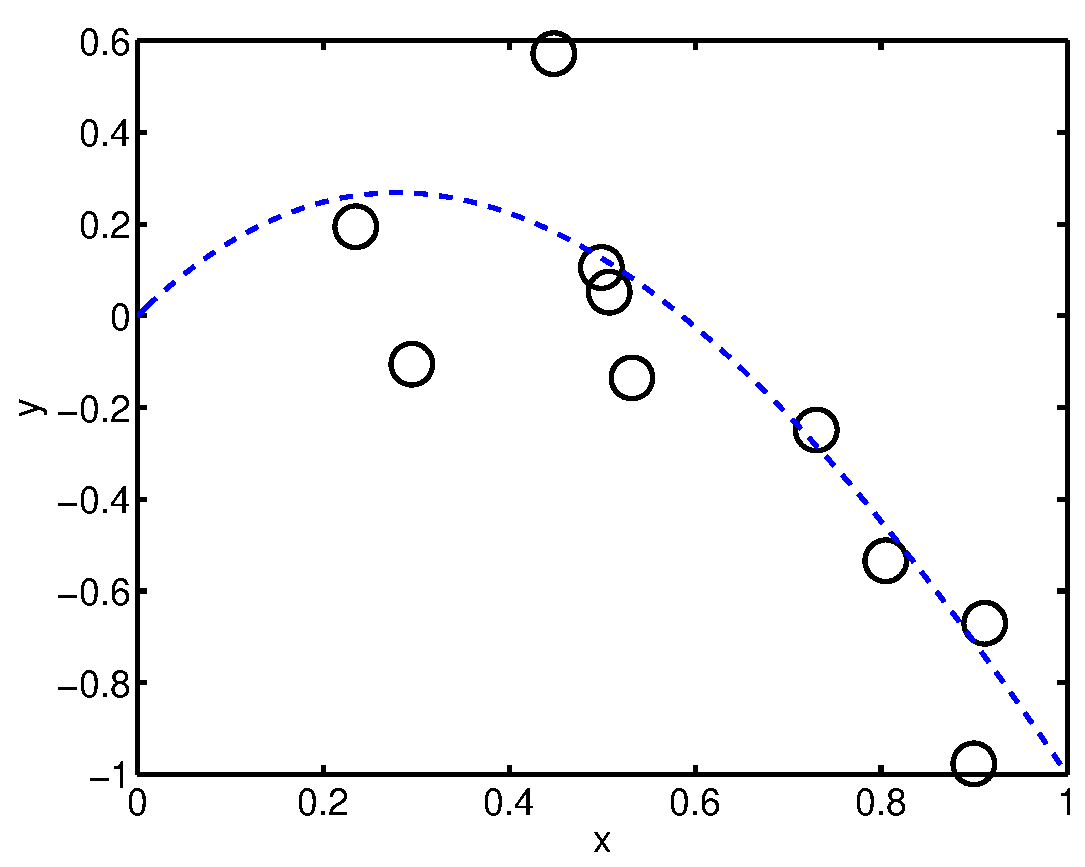
\includegraphics[width=0.7\linewidth]{gpintro_data.pdf}		
		\centering\caption{\label{fig:gpintro_data}A familiar problem: learn the underlying function (blue) from the observed data (crosses).}
	\end{figure}
\end{frame}

\begin{frame}
	\frametitle{A parametric approach?}
	\begin{figure}[tbh]
		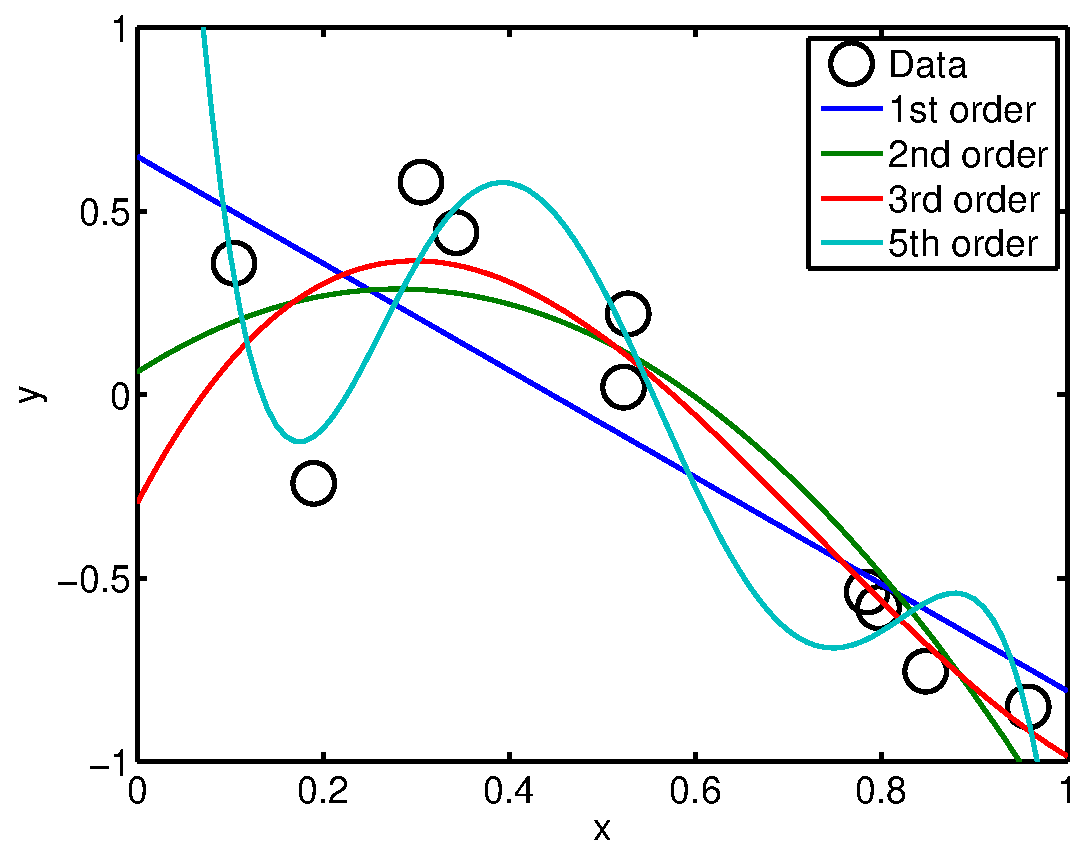
\includegraphics[width=0.7\linewidth]{gpintro_poly.pdf}		
		\centering\caption{\label{fig:gpintro_poly}Polynomials fitted by least squares.}
		It's easy to under and over-fit. What if we have no idea of the parametric form of the function?
	\end{figure}
\end{frame}

\begin{frame}
	\frametitle{A non-parametric approach - Gaussian Processes}
	\begin{itemize}
		\item Rather than forcing us to choose a particular parametric form, a \ac{GP} allows us to place a prior distribution directly on \emph{functions}
		\item With a \ac{GP} prior we can:
		\begin{itemize}
			\item Sample functions from the prior
			\item Incorporate data to get a \emph{posterior} distribution over functions
			\item Make predictions
		\end{itemize}
	\end{itemize}
\end{frame}

\begin{frame}
	\frametitle{Visual example -- prior}
	\begin{figure}[tbh]
		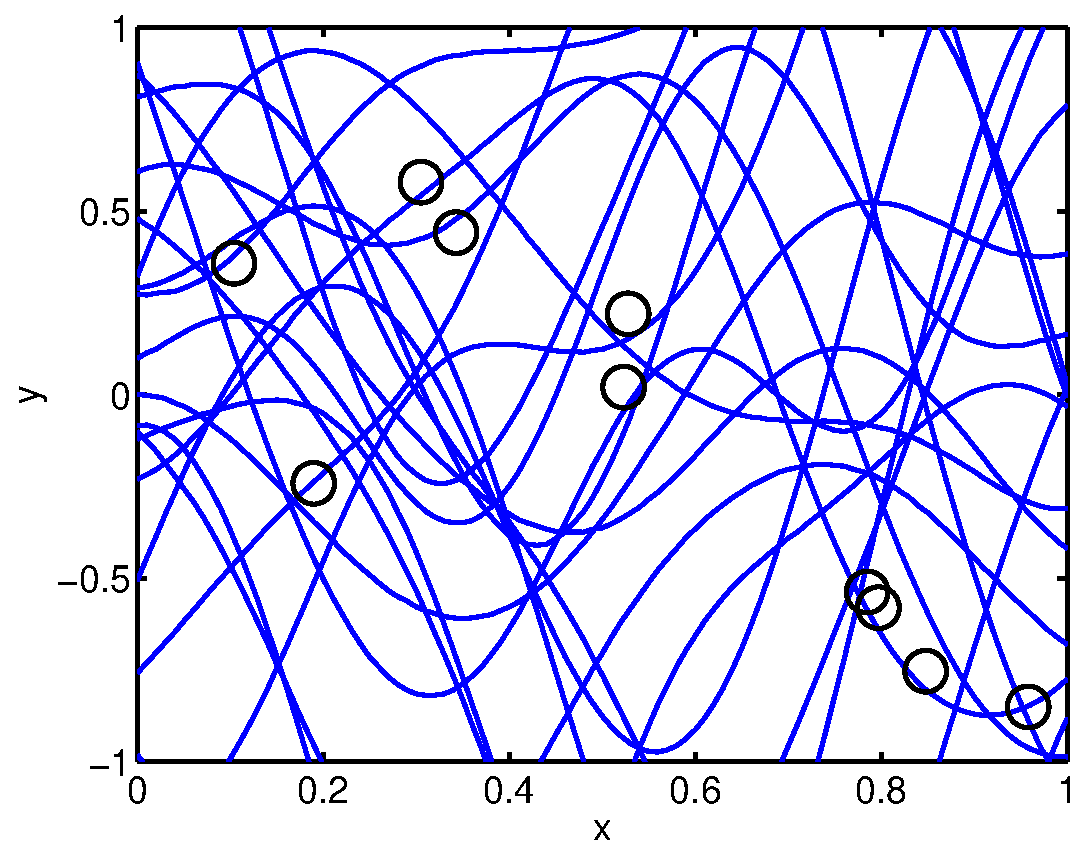
\includegraphics[width=0.7\linewidth]{gpintro_prior.pdf}		
		\centering\caption{\label{fig:gpintro_prior}Some functions drawn from a \ac{GP} prior.}
	\end{figure}
\end{frame}

\begin{frame}
	\frametitle{Visual exmample -- posterior}
	\begin{figure}[tbh]
		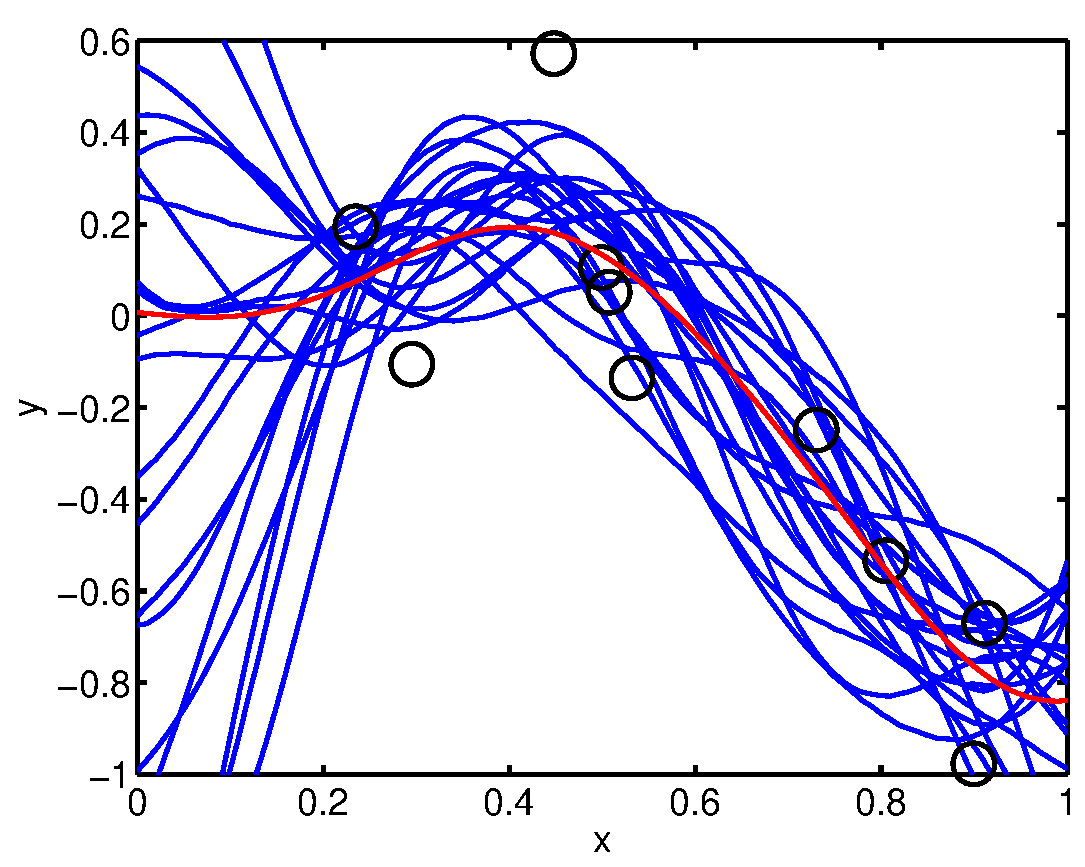
\includegraphics[width=0.7\linewidth]{gpintro_posterior.pdf}		
		\centering\caption{\label{fig:gpintro_posterior}Some functions drawn from the \ac{GP} posterior. Posterior mean is shown in red.}
	\end{figure}
\end{frame}

\begin{frame}
	\frametitle{Visual example -- predictions}
	\begin{figure}[tbh]
		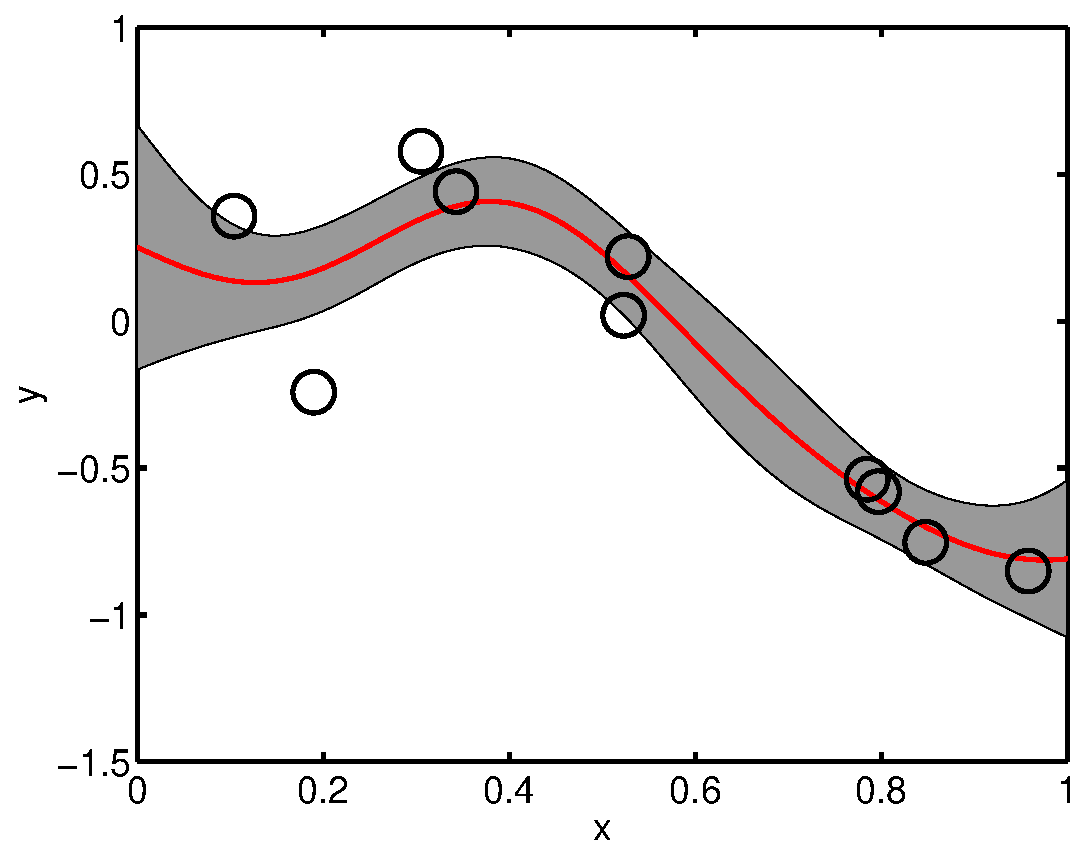
\includegraphics[width=0.7\linewidth]{gpintro_predictions.pdf}		
		\centering\caption{\label{fig:gpintro_predictions.pdf}Predictive mean and standard deviations.}
	\end{figure}
\end{frame}

\begin{frame}
	\frametitle{Some formalities}
	\begin{itemize}
		\item We observe $N$ training points, each of which consists of a set of features $\bx_n$ and a target $y_n$.
		\item We can stack all of the $y_n$ into a vector and $\bx_n$ into a matrix:
		\[
		\by = \left[
			\begin{array}{c}
			y_1 \\ y_2 \\ \vdots \\ y_N
			\end{array}
		\right],~~~
		\bX = \left[
		\begin{array}{c}
			\bx_1^T \\ \bx_2^T \\ \vdots \\ \bx_N^T
		\end{array}
		\right]
		\]
	\end{itemize}

\end{frame}

\begin{frame}
	\frametitle{GP definition}
	\begin{itemize}
		\item The GP assumes that the vector of \emph{all possible} $y_n$ is a draw from a \ac{MVG}.
		\item We don't observe \emph{all possible} values (if we did, we wouldn't need to make predictions!)
		\visible<2->{\item But the marginal densities of a \ac{MVG} are also \ac{MVG}s so the subset we observe are also a draw from a \ac{MVG}.
		\[
			\by \sim {\cal N}(\boldsymbol\mu,\mathbf{C})
		\]
		\item i.e. if we have $N$ training points, we're dealing with an $N$-dimensional \ac{MVG}}
		\visible<3->{\item With mean $\boldsymbol\mu$ (normally 0) and covariance $\mathbf{C}$} 
		\visible<4->{\item $\bx_n$ looks to have disappeared -- we find it inside $\mathbf{C}$}
	\end{itemize}
\end{frame}

\begin{frame}
	\frametitle{GP definition}
	\begin{figure}[tbh]
		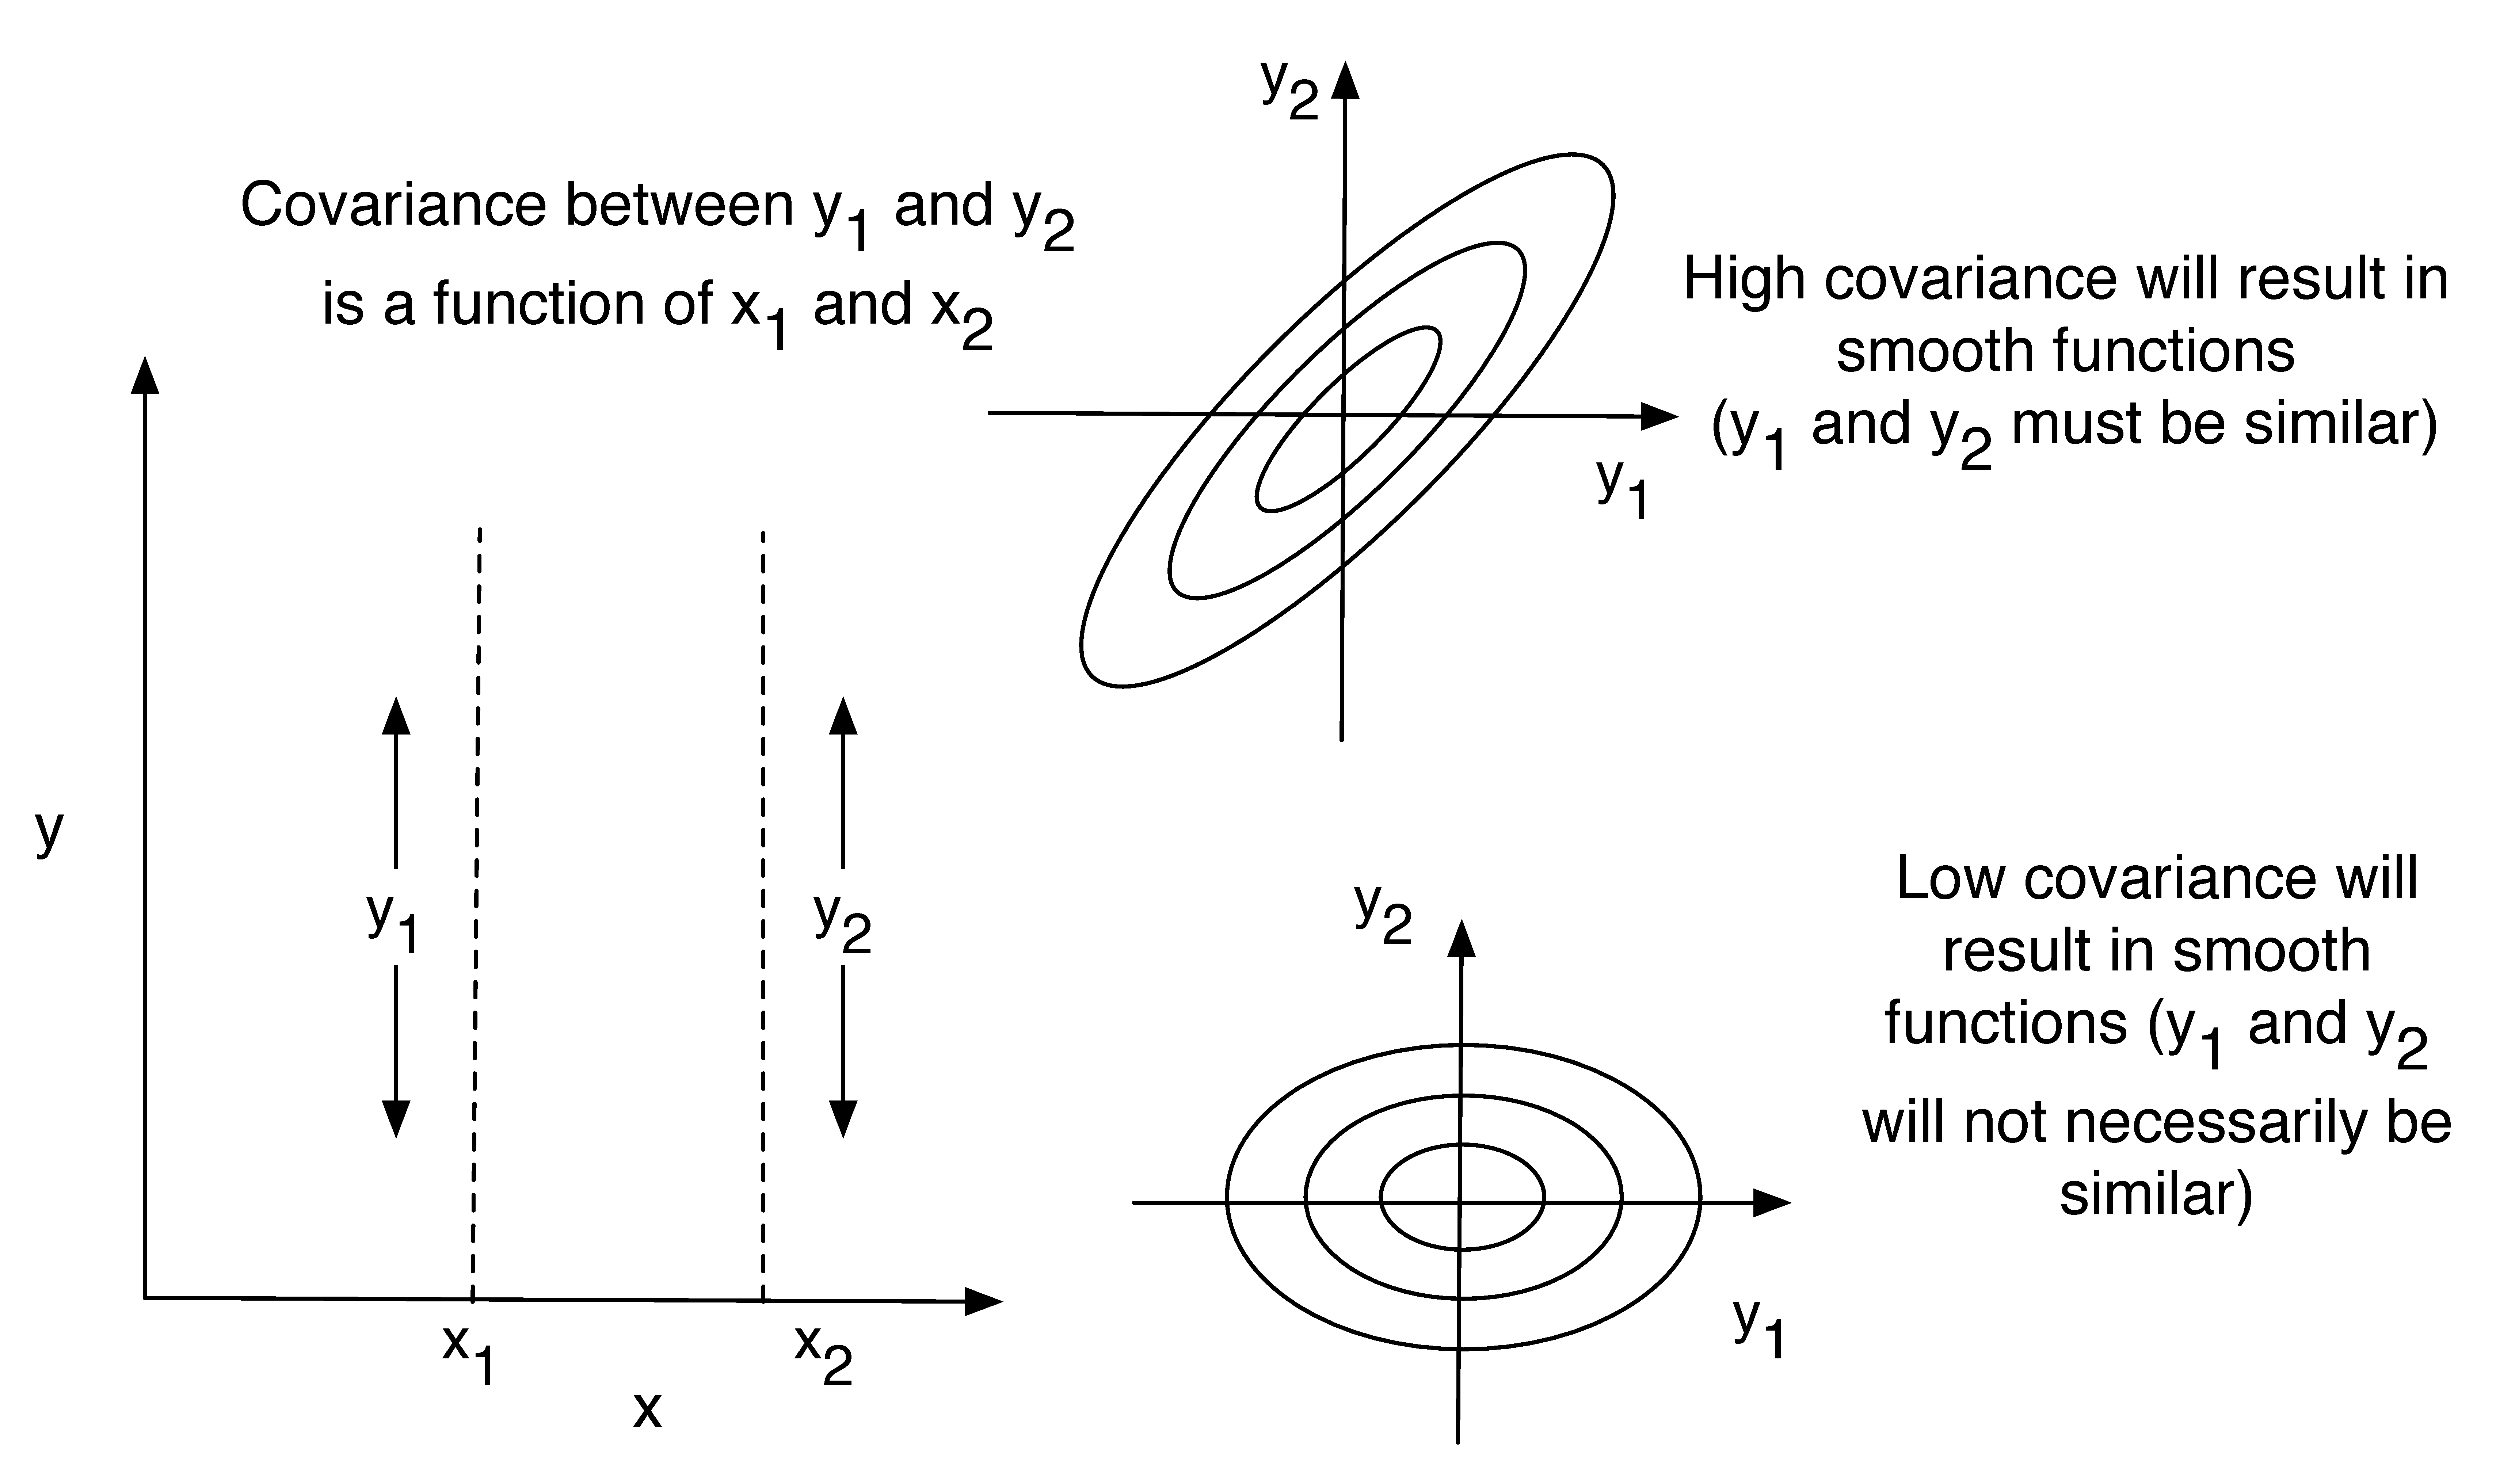
\includegraphics[width=\linewidth]{GPcartoon.pdf}		
		\centering\caption{\label{fig:GPcartoon}Schematic of GP prior for two function values.}
	\end{figure}
\end{frame}


\begin{frame}
	\frametitle{Covariance functions}
	\begin{itemize}
		\item By choosing a covariance function, we are making an assumption on the \emph{smoothness} of the regression function.
		\item Common choices:
		\begin{itemize}
			\item Linear: $C(\bx_1,\bx_2) = \bx_1^T\bx_2$
			\item RBF: $C(\bx_1,\bx_2) = \exp\left\{-0.5\gamma ||\bx_1 - \bx_2||^2 \right\}$
			\item And many, many more.
		\end{itemize}
		\item More details: \url{http://www.gaussianprocess.org/gpml/}
		\begin{itemize}
			\item (Free) book
			\item Code
		\end{itemize}
	\end{itemize}
\end{frame}

\begin{frame}
	\frametitle{Hyper-parameters}
	\[
C(\bx_1,\bx_2) = \exp\left\{-0.5\gamma ||\bx_1 - \bx_2||^2 \right\}
	\]
	\begin{figure}[tbh]
		\subfigure[$\gamma=1$]{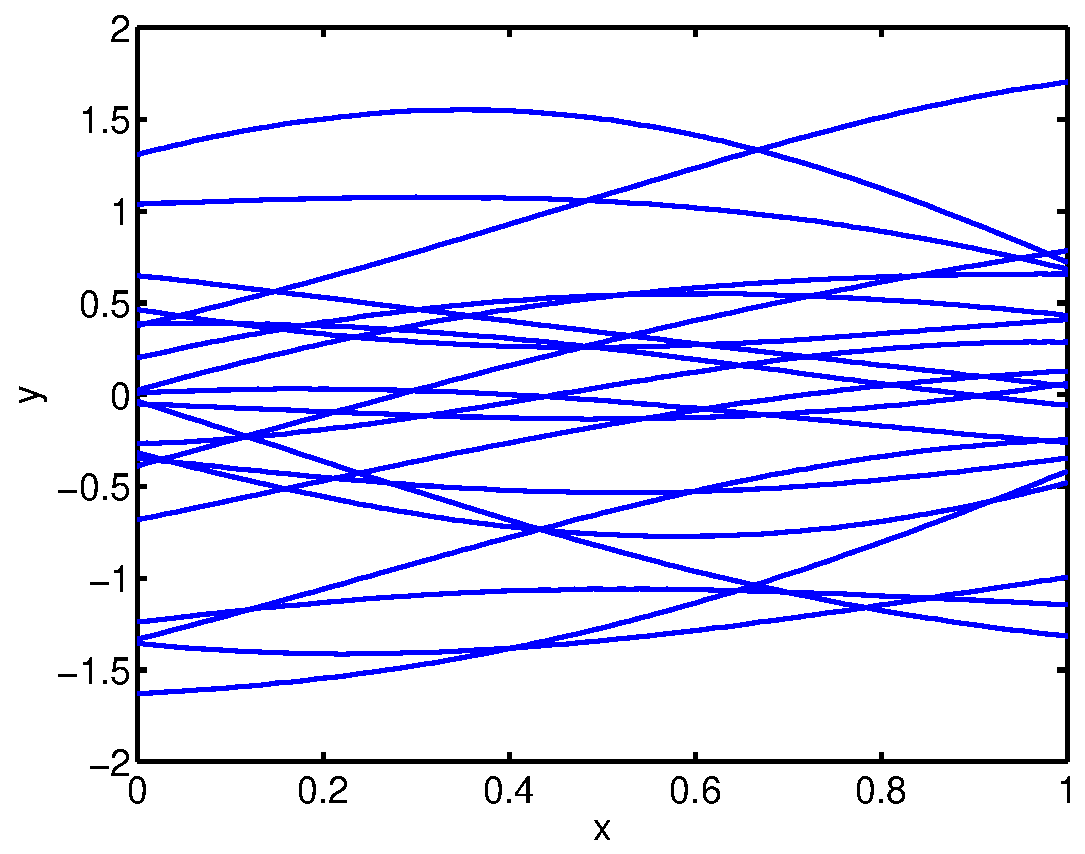
\includegraphics[width=0.32\linewidth]{gpintro_prior_hyp1.pdf}}
		\subfigure[$\gamma=10$]{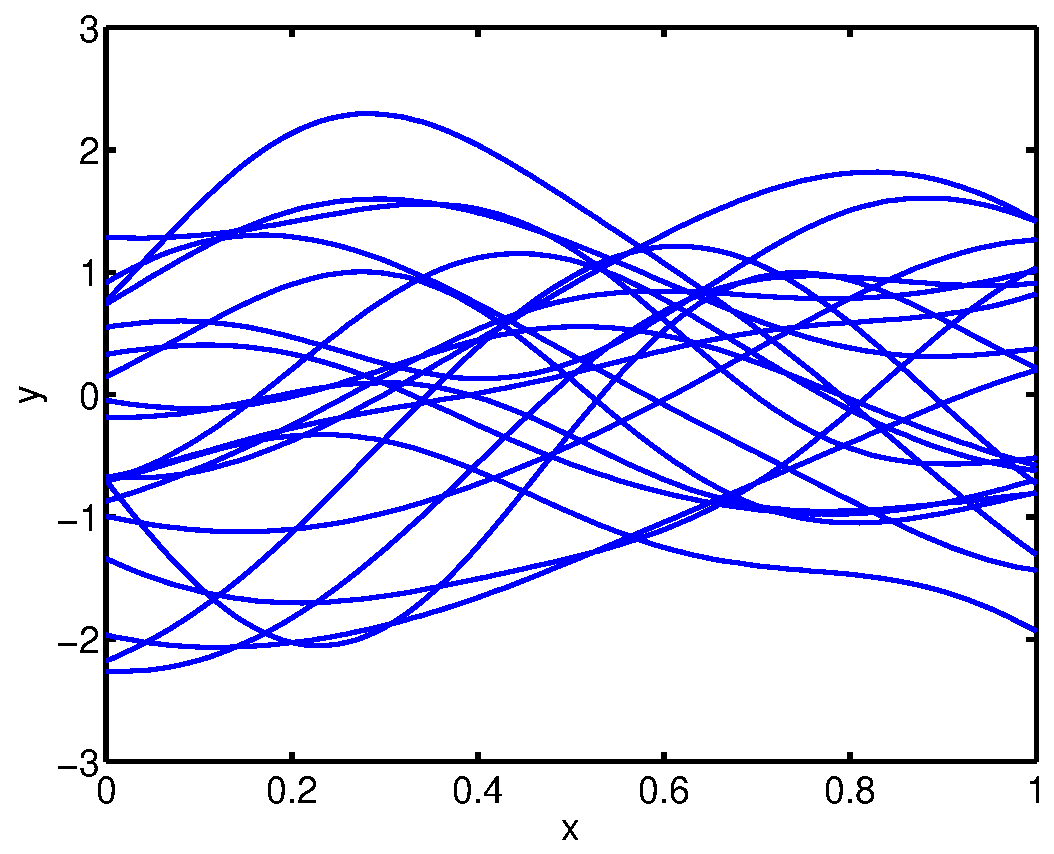
\includegraphics[width=0.32\linewidth]{gpintro_prior_hyp10.pdf}}
		\subfigure[$\gamma=100$]{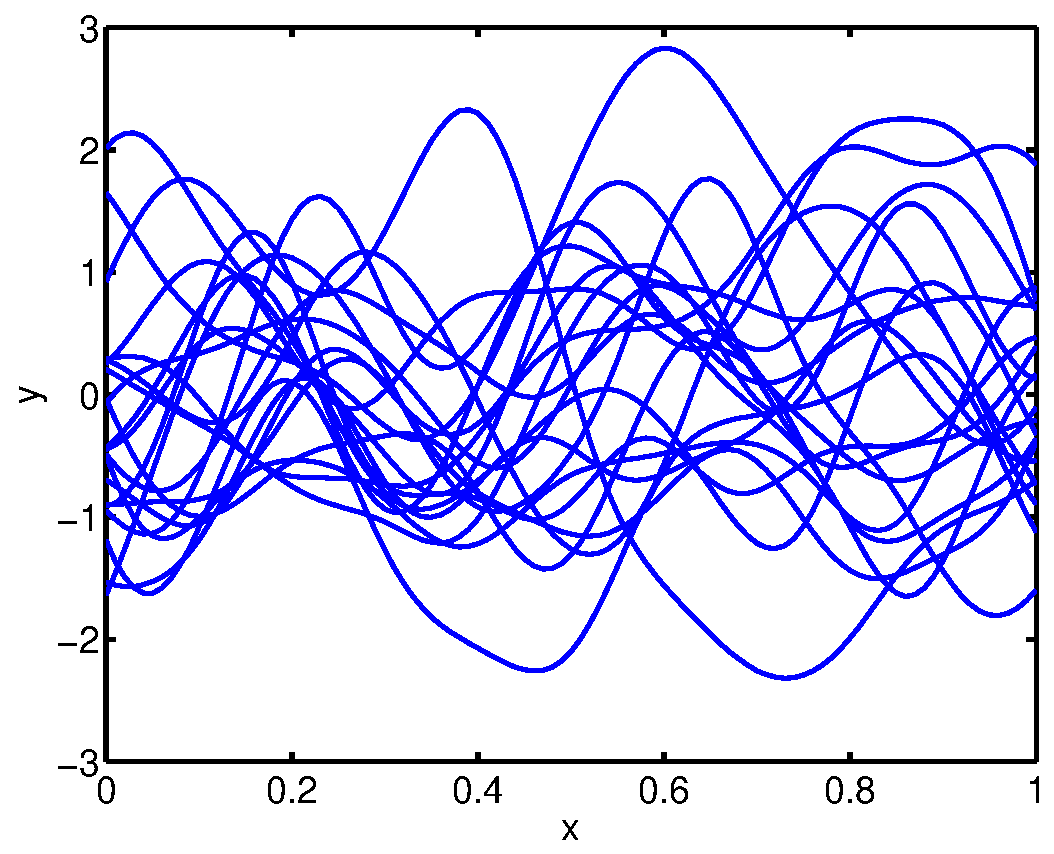
\includegraphics[width=0.32\linewidth]{gpintro_prior_hyp100.pdf}}
		\centering\caption{\label{fig:hyper}Varying hyper-parameters in an RBF covariance varies the smoothness of the function.}
	\end{figure}
\end{frame}

\begin{frame}
	\frametitle{Optimising hyper-parameters}
	
\end{frame}

\begin{frame}
	\frametitle{Making predictions}
	\begin{itemize}
		\item If we assume no observation noise, we can place \ac{GP} prior directly on $\by$
		\item If we observe $\by$ and want to predict $y_*$ for a new observation $\bx_*$:
		\begin{itemize}
			\item Construct joint Density (it's a Gaussian):
			\[
				\left[
					\begin{array}{c}
						\by \\ y_*
					\end{array}
				\right]
				\sim 
				{\cal N} 	\left (
								\mathbf{0} , 
								\left [
									\begin{array}{cc}
											C(\bX,\bX) & C(\bX,\bx_*) \\ 
											C(\bx_*,\bX) & C(\bx_*,\bx_*)
									\end{array}
								\right ]
							\right )
			\]
			\item And then use standard results for Gaussian conditionals:
			\[
				p(y_*|\by,\bX,\bx_*) = {\cal N}(\mu_*,\sigma^2_*)
			\]
			where
			\begin{eqnarray}
				\nonumber \mu_* &=& C(\bx_*,\bX)C(\bX,\bX)^{-1}\by\\
				\nonumber \sigma^2_* &=& C(\bx_*,\bx_*) - C(\bx_*,\bX)C(\bX,\bX)^{-1}K(\bX,\bx^*)
			\end{eqnarray}
		\end{itemize}
	\end{itemize}
	{\small \url{http://orion.uwaterloo.ca/~hwolkowi/matrixcookbook.pdf}}
\end{frame}

\begin{frame}
	\frametitle{Noise-free example}
	\begin{figure}[tbh]
		\centering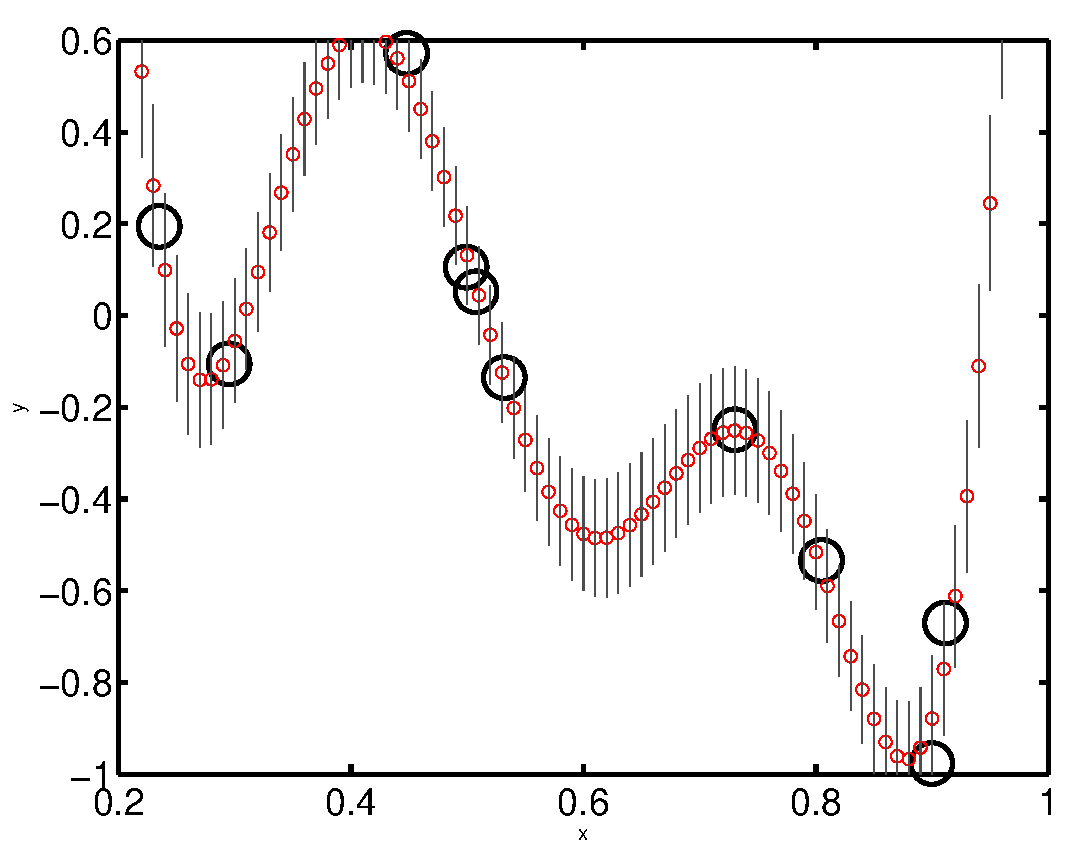
\includegraphics[width=0.7\linewidth]{gpintro_noisefree.pdf}
		\centering\caption{\label{fig:gpintro_noisefree}$\mu_*\pm \sigma_*$ for a noise-free GP at lots of test points}
	\end{figure}
\end{frame}

\begin{frame}
	\frametitle{Predictions with noise}
	\begin{itemize}
		\item Assuming Gaussian observation noise, we introduce a set of latent variables, $f_n$ and place the GP prior on these.
		\[
			y_n \sim {\cal N}(f_n,\sigma^2),~~ \blf \sim {\cal N}(\mathbf{0},\mathbf{C})
		\]
		\visible<2->{
			\item Because both terms are Gaussian, the noise can be pushed into the covariance function:
			\[
				\left[
					\begin{array}{c}
						\by \\ f_*
					\end{array}
				\right]
				\sim 
				{\cal N} 	\left (
								\mathbf{0} , 
								\left [
									\begin{array}{cc}
											C(\bX,\bX) + \sigma^2\mathbf{I} & C(\bX,\bx_*) \\ 
											C(\bx_*,\bX) & C(\bx_*,\bx_*)
									\end{array}
								\right ]
							\right )
			\]
		}
		\visible<3->{
			\item And, as before (except now predicting $f_*$):
			\[
				p(f_*|\by,\bX,\bx_*,\sigma^2) = {\cal N}(\mu_*,\sigma^2_*)
			\]
			where
			\begin{eqnarray}
				\nonumber \mu_* &=& C(\bx_*,\bX)\left[C(\bX,\bX)+\sigma^2\mathbf{I}\right]^{-1}\by\\
				\nonumber \sigma^2_* &=& C(\bx_*,\bx_*) - C(\bx_*,\bX)\left[C(\bX,\bX)+\sigma^2\mathbf{I}\right]^{-1}K(\bX,\bx^*)
			\end{eqnarray}
		}
	\end{itemize}
\end{frame}


\begin{frame}
	\frametitle{Example with noise}
	\begin{figure}[tbh]
		\centering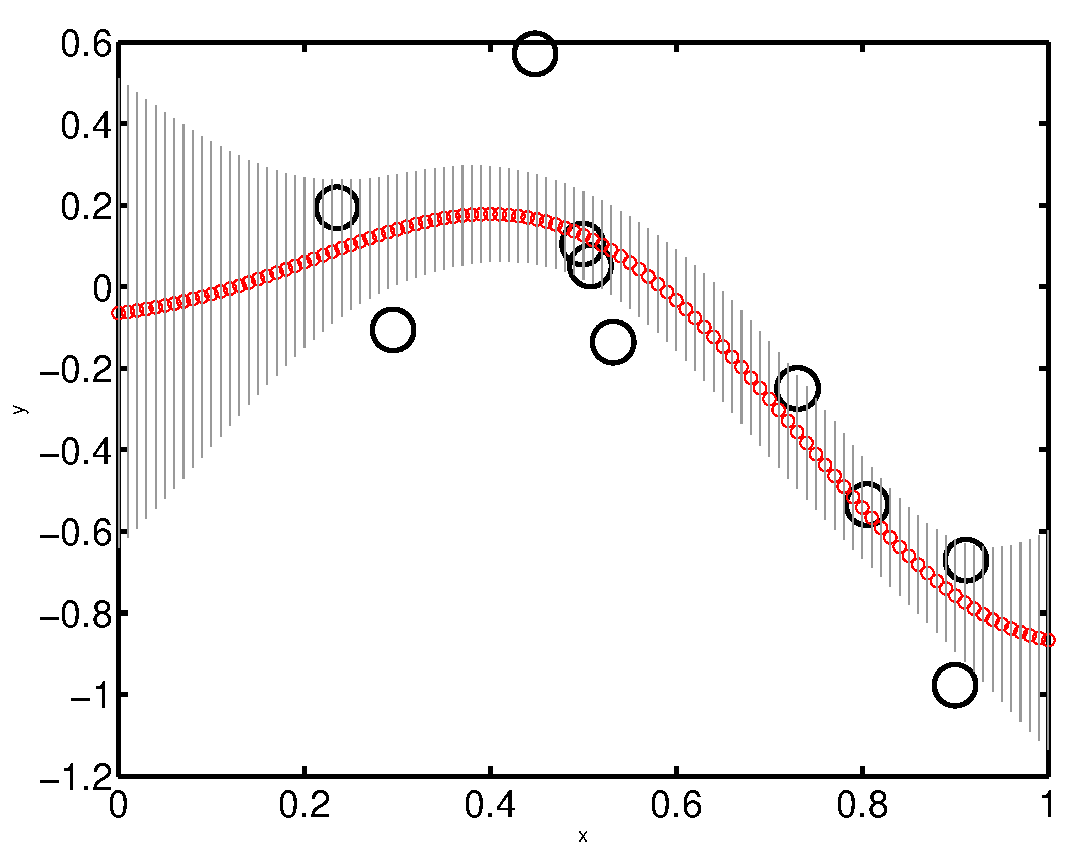
\includegraphics[width=0.7\linewidth]{gpintro_withnoise.pdf}
		\centering\caption{\label{fig:gpintro_withnoise}$\mu_*\pm\sigma_*$ at lots of test points when observation noise is included.}
	\end{figure}
\end{frame}

